\section*{Introduction}

This report explains the implementation details of CS523 Computer Vision Assignment 1, which is about detecting rectangles in a given sudoku puzzle image. The pre-processing of the given image will be explained first and will be followed by the logic behind the rectangle extraction. Lastly, I will add my findings and comments. To run the code, there needs to be a directory which contains the .jpg files. The directory and main.py needs to be at the same level. 


\section*{Pre-Processing}

After examining the pictures in the dataset, I decided to pre-process the image to clear some of the noise so that the detector will perform better. Since we do not need the color information, I first downsampled the image by converting it to gray-scale. Once I got a gray-scale image, I applied a Gaussian Blur to remove some noise and make the extraction of the grid easier. After lots of trials and errors, I decided to use a Kernel size of 5x5 for Gaussian Blur. Afterwards, I applied a
thresholding algorithm. The idea behind thresholding is that if a pixel has a value smaller than a threshold, it is set to 0, otherwise it is set to a maximum value. Since the images in the dataset had different illumination levels, instead of a global thresholding, I used adaptive thresholding, which determines the threshold for a pixel based on a small region around it.

\begin{figure}[H]
    \centering
    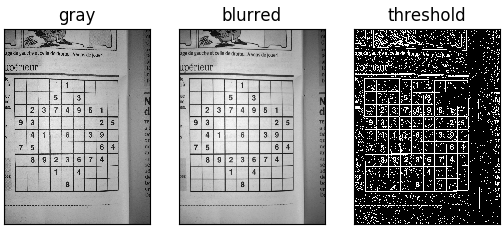
\includegraphics[width=\textwidth]{images/preprocess.png}
    \caption{Phases of the image during pre-processing}
    \setlength{\belowcaptionskip}{-20pt}
    \setlength{\abovecaptionskip}{-20pt}
\end{figure}

\newpage

\section*{Detecting The Biggest Blob}

Now that I have my image ready for rectangle detection, I assumed that the biggest polygon in the image is the sudoku grid. I found all the contours in the image using cv2.findContours method. I sorted the contours with respect to their areas and got the biggest blob.

\begin{figure}[H]
    \centering
    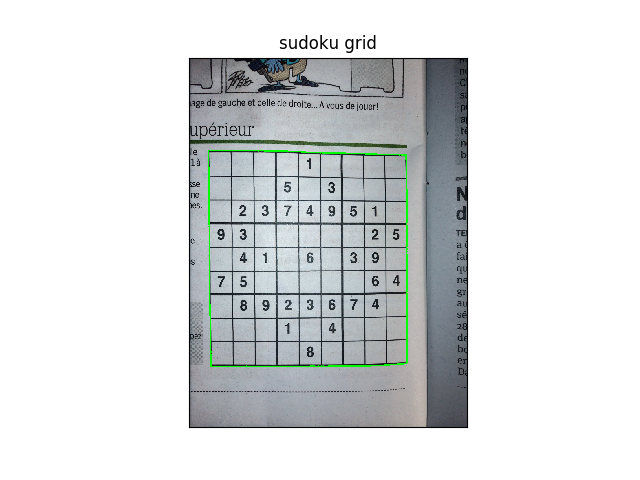
\includegraphics[width=\textwidth]{images/extracted_grid.png}
    \caption{Biggest Blob of the image}
    \setlength{\belowcaptionskip}{-20pt}
    \setlength{\abovecaptionskip}{-20pt}
\end{figure}

\newpage

\section*{Detecting The Sudoku Cells}

With the detected borders of the Sudoku grid, I created a mask image to only focus on what is inside the Sudoku Grid. I created a new image and cropped it with the help of the mask, so that I have a region of interest. Just like the pre-processing phase, I applied Gaussian Blur and adaptive thresholding, this time to make the image ready for the detection of smaller rectangles. For images with a higher quality, I used a kernel size with 11x11, I found out that for images with bad quality
smaller sized kernels performed better.

\begin{figure}[H]
    \centering
    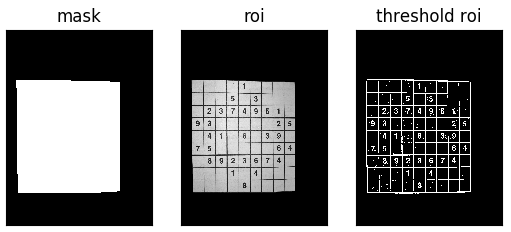
\includegraphics[width=\textwidth]{images/masked.png}
    \caption{Phases of the image after applying the mask}
    \setlength{\belowcaptionskip}{-20pt}
    \setlength{\abovecaptionskip}{-20pt}
\end{figure}

Now, I have the image ready for the detection of the sudoku cells. Again, after some trial and error, I figured out that if the area of a contour is bigger than 800, it is a cell in the sudoku grid.

\begin{figure}[H]
    \centering
    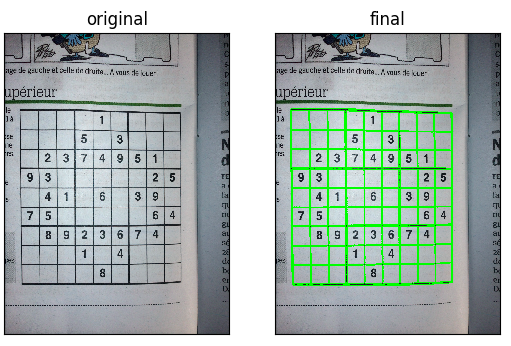
\includegraphics[width=\textwidth]{images/final.png}
    \caption{Processed image}
    \setlength{\belowcaptionskip}{-20pt}
    \setlength{\abovecaptionskip}{-20pt}
\end{figure}

\section*{Findings \& Comments}
There were 40 images in the v2\_dataset. My algorithm successfully detected all the cells in the sudoku grid in 17 of the images, only the bounding rectangle with some missing cells in 8 images and detected only some of the cells in 16 images. I believe my results are not bad considering the quality of the images in the dataset. The algorithm can also I also tried using HoughLines for the detection of the lines but I was not satisfied with the overall results and ended up using processing the contours.
\begin{figure}[H]
    \centering
    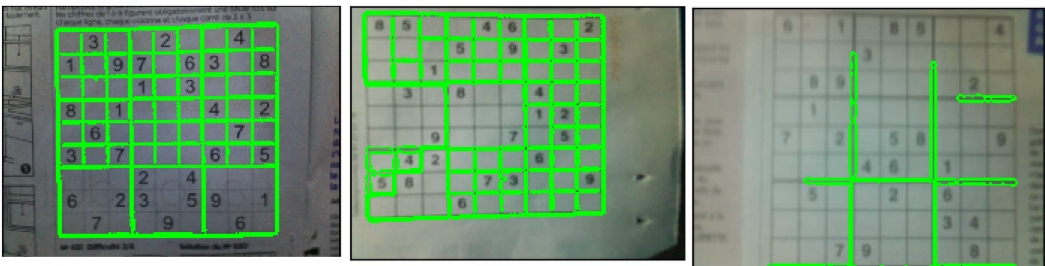
\includegraphics[width=\textwidth]{images/bad_images.png}
    \caption{Unsuccessful Results}
    \setlength{\belowcaptionskip}{-20pt}
    \setlength{\abovecaptionskip}{-20pt}
\end{figure}

